\documentclass[1p]{elsarticle_modified}
%\bibliographystyle{elsarticle-num}

%\usepackage[colorlinks]{hyperref}
%\usepackage{abbrmath_seonhwa} %\Abb, \Ascr, \Acal ,\Abf, \Afrak
\usepackage{amsfonts}
\usepackage{amssymb}
\usepackage{amsmath}
\usepackage{amsthm}
\usepackage{scalefnt}
\usepackage{amsbsy}
\usepackage{kotex}
\usepackage{caption}
\usepackage{subfig}
\usepackage{color}
\usepackage{graphicx}
\usepackage{xcolor} %% white, black, red, green, blue, cyan, magenta, yellow
\usepackage{float}
\usepackage{setspace}
\usepackage{hyperref}

\usepackage{tikz}
\usetikzlibrary{arrows}

\usepackage{multirow}
\usepackage{array} % fixed length table
\usepackage{hhline}

%%%%%%%%%%%%%%%%%%%%%
\makeatletter
\renewcommand*\env@matrix[1][\arraystretch]{%
	\edef\arraystretch{#1}%
	\hskip -\arraycolsep
	\let\@ifnextchar\new@ifnextchar
	\array{*\c@MaxMatrixCols c}}
\makeatother %https://tex.stackexchange.com/questions/14071/how-can-i-increase-the-line-spacing-in-a-matrix
%%%%%%%%%%%%%%%

\usepackage[normalem]{ulem}

\newcommand{\msout}[1]{\ifmmode\text{\sout{\ensuremath{#1}}}\else\sout{#1}\fi}
%SOURCE: \msout is \stkout macro in https://tex.stackexchange.com/questions/20609/strikeout-in-math-mode

\newcommand{\cancel}[1]{
	\ifmmode
	{\color{red}\msout{#1}}
	\else
	{\color{red}\sout{#1}}
	\fi
}

\newcommand{\add}[1]{
	{\color{blue}\uwave{#1}}
}

\newcommand{\replace}[2]{
	\ifmmode
	{\color{red}\msout{#1}}{\color{blue}\uwave{#2}}
	\else
	{\color{red}\sout{#1}}{\color{blue}\uwave{#2}}
	\fi
}

\newcommand{\Sol}{\mathcal{S}} %segment
\newcommand{\D}{D} %diagram
\newcommand{\A}{\mathcal{A}} %arc


%%%%%%%%%%%%%%%%%%%%%%%%%%%%%5 test

\def\sl{\operatorname{\textup{SL}}(2,\Cbb)}
\def\psl{\operatorname{\textup{PSL}}(2,\Cbb)}
\def\quan{\mkern 1mu \triangleright \mkern 1mu}

\theoremstyle{definition}
\newtheorem{thm}{Theorem}[section]
\newtheorem{prop}[thm]{Proposition}
\newtheorem{lem}[thm]{Lemma}
\newtheorem{ques}[thm]{Question}
\newtheorem{cor}[thm]{Corollary}
\newtheorem{defn}[thm]{Definition}
\newtheorem{exam}[thm]{Example}
\newtheorem{rmk}[thm]{Remark}
\newtheorem{alg}[thm]{Algorithm}

\newcommand{\I}{\sqrt{-1}}
\begin{document}

%\begin{frontmatter}
%
%\title{Boundary parabolic representations of knots up to 8 crossings}
%
%%% Group authors per affiliation:
%\author{Yunhi Cho} 
%\address{Department of Mathematics, University of Seoul, Seoul, Korea}
%\ead{yhcho@uos.ac.kr}
%
%
%\author{Seonhwa Kim} %\fnref{s_kim}}
%\address{Center for Geometry and Physics, Institute for Basic Science, Pohang, 37673, Korea}
%\ead{ryeona17@ibs.re.kr}
%
%\author{Hyuk Kim}
%\address{Department of Mathematical Sciences, Seoul National University, Seoul 08826, Korea}
%\ead{hyukkim@snu.ac.kr}
%
%\author{Seokbeom Yoon}
%\address{Department of Mathematical Sciences, Seoul National University, Seoul, 08826,  Korea}
%\ead{sbyoon15@snu.ac.kr}
%
%\begin{abstract}
%We find all boundary parabolic representation of knots up to 8 crossings.
%
%\end{abstract}
%\begin{keyword}
%    \MSC[2010] 57M25 
%\end{keyword}
%
%\end{frontmatter}

%\linenumbers
%\tableofcontents
%
\newcommand\colored[1]{\textcolor{white}{\rule[-0.35ex]{0.8em}{1.4ex}}\kern-0.8em\color{red} #1}%
%\newcommand\colored[1]{\textcolor{white}{ #1}\kern-2.17ex	\textcolor{white}{ #1}\kern-1.81ex	\textcolor{white}{ #1}\kern-2.15ex\color{red}#1	}

{\Large $\underline{11a_{172}~(K11a_{172})}$}

\setlength{\tabcolsep}{10pt}
\renewcommand{\arraystretch}{1.6}
\vspace{1cm}\begin{tabular}{m{100pt}>{\centering\arraybackslash}m{274pt}}
\multirow{5}{120pt}{
	\centering
	\includegraphics[width=112pt]{../../../GIT/diagram.site/Diagrams/png/421_11a_172.png}\\
\ \ \ A knot diagram\footnotemark}&
\allowdisplaybreaks
\textbf{Linearized knot diagam} \\
\cline{2-2}
 &
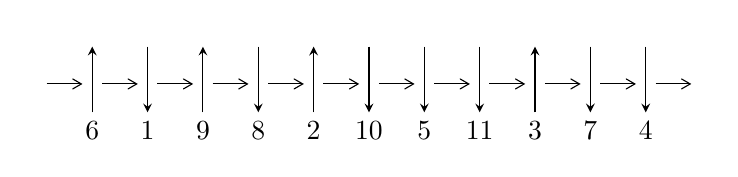
\begin{tikzpicture}[x=20pt, y=17pt]
	% nodes
	\node (C0) at (0, 0) {};
	\node (C1) at (1, 0) {};
	\node (C1U) at (1, +1) {};
	\node (C1D) at (1, -1) {6};

	\node (C2) at (2, 0) {};
	\node (C2U) at (2, +1) {};
	\node (C2D) at (2, -1) {1};

	\node (C3) at (3, 0) {};
	\node (C3U) at (3, +1) {};
	\node (C3D) at (3, -1) {9};

	\node (C4) at (4, 0) {};
	\node (C4U) at (4, +1) {};
	\node (C4D) at (4, -1) {8};

	\node (C5) at (5, 0) {};
	\node (C5U) at (5, +1) {};
	\node (C5D) at (5, -1) {2};

	\node (C6) at (6, 0) {};
	\node (C6U) at (6, +1) {};
	\node (C6D) at (6, -1) {10};

	\node (C7) at (7, 0) {};
	\node (C7U) at (7, +1) {};
	\node (C7D) at (7, -1) {5};

	\node (C8) at (8, 0) {};
	\node (C8U) at (8, +1) {};
	\node (C8D) at (8, -1) {11};

	\node (C9) at (9, 0) {};
	\node (C9U) at (9, +1) {};
	\node (C9D) at (9, -1) {3};

	\node (C10) at (10, 0) {};
	\node (C10U) at (10, +1) {};
	\node (C10D) at (10, -1) {7};

	\node (C11) at (11, 0) {};
	\node (C11U) at (11, +1) {};
	\node (C11D) at (11, -1) {4};
	\node (C12) at (12, 0) {};

	% arrows
	\draw[->,>={angle 60}]
	(C0) edge (C1) (C1) edge (C2) (C2) edge (C3) (C3) edge (C4) (C4) edge (C5) (C5) edge (C6) (C6) edge (C7) (C7) edge (C8) (C8) edge (C9) (C9) edge (C10) (C10) edge (C11) (C11) edge (C12) ;	\draw[->,>=stealth]
	(C1D) edge (C1U) (C2U) edge (C2D) (C3D) edge (C3U) (C4U) edge (C4D) (C5D) edge (C5U) (C6U) edge (C6D) (C7U) edge (C7D) (C8U) edge (C8D) (C9D) edge (C9U) (C10U) edge (C10D) (C11U) edge (C11D) ;
	\end{tikzpicture} \\
\hhline{~~} \\& 
\textbf{Solving Sequence} \\ \cline{2-2} 
 &
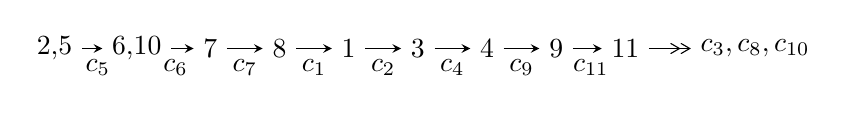
\begin{tikzpicture}[x=25pt, y=7pt]
	% node
	\node (A0) at (-1/8, 0) {2,5};
	\node (A1) at (17/16, 0) {6,10};
	\node (A2) at (17/8, 0) {7};
	\node (A3) at (25/8, 0) {8};
	\node (A4) at (33/8, 0) {1};
	\node (A5) at (41/8, 0) {3};
	\node (A6) at (49/8, 0) {4};
	\node (A7) at (57/8, 0) {9};
	\node (A8) at (65/8, 0) {11};
	\node (C1) at (1/2, -1) {$c_{5}$};
	\node (C2) at (13/8, -1) {$c_{6}$};
	\node (C3) at (21/8, -1) {$c_{7}$};
	\node (C4) at (29/8, -1) {$c_{1}$};
	\node (C5) at (37/8, -1) {$c_{2}$};
	\node (C6) at (45/8, -1) {$c_{4}$};
	\node (C7) at (53/8, -1) {$c_{9}$};
	\node (C8) at (61/8, -1) {$c_{11}$};
	\node (A9) at (10, 0) {$c_{3},c_{8},c_{10}$};

	% edge
	\draw[->,>=stealth]	
	(A0) edge (A1) (A1) edge (A2) (A2) edge (A3) (A3) edge (A4) (A4) edge (A5) (A5) edge (A6) (A6) edge (A7) (A7) edge (A8) ;
	\draw[->>,>={angle 60}]	
	(A8) edge (A9);
\end{tikzpicture} \\ 

\end{tabular} \\

\footnotetext{
The image of knot diagram is generated by the software ``\textbf{Draw programme}" developed by Andrew Bartholomew(\url{http://www.layer8.co.uk/maths/draw/index.htm\#Running-draw}), where we modified some parts for our purpose(\url{https://github.com/CATsTAILs/LinksPainter}).
}\phantom \\ \newline 
\centering \textbf{Ideals for irreducible components\footnotemark of $X_{\text{par}}$} 
 
\begin{align*}
I^u_{1}&=\langle 
-2.51962\times10^{120} u^{80}+2.58128\times10^{120} u^{79}+\cdots+2.77111\times10^{119} b+2.51695\times10^{121},\\
\phantom{I^u_{1}}&\phantom{= \langle  }1.23775\times10^{121} u^{80}+2.60882\times10^{121} u^{79}+\cdots+3.04822\times10^{120} a+3.89021\times10^{122},\\
\phantom{I^u_{1}}&\phantom{= \langle  }u^{81}- u^{80}+\cdots+146 u+11\rangle \\
I^u_{2}&=\langle 
u^{10}+2 u^9+5 u^8+6 u^7+10 u^6+9 u^5+12 u^4+5 u^3+8 u^2+b+u+3,\\
\phantom{I^u_{2}}&\phantom{= \langle  }3 u^{10}+5 u^9+12 u^8+12 u^7+21 u^6+15 u^5+24 u^4+5 u^3+16 u^2+a+u+6,\\
\phantom{I^u_{2}}&\phantom{= \langle  }u^{12}+2 u^{11}+5 u^{10}+6 u^9+10 u^8+9 u^7+13 u^6+7 u^5+10 u^4+3 u^3+5 u^2+u+1\rangle \\
\\
\end{align*}
\raggedright * 2 irreducible components of $\dim_{\mathbb{C}}=0$, with total 93 representations.\\
\footnotetext{All coefficients of polynomials are rational numbers. But the coefficients are sometimes approximated in decimal forms when there is not enough margin.}
\newpage
\renewcommand{\arraystretch}{1}
\centering \section*{I. $I^u_{1}= \langle -2.52\times10^{120} u^{80}+2.58\times10^{120} u^{79}+\cdots+2.77\times10^{119} b+2.52\times10^{121},\;1.24\times10^{121} u^{80}+2.61\times10^{121} u^{79}+\cdots+3.05\times10^{120} a+3.89\times10^{122},\;u^{81}- u^{80}+\cdots+146 u+11 \rangle$}
\flushleft \textbf{(i) Arc colorings}\\
\begin{tabular}{m{7pt} m{180pt} m{7pt} m{180pt} }
\flushright $a_{2}=$&$\begin{pmatrix}0\\u\end{pmatrix}$ \\
\flushright $a_{5}=$&$\begin{pmatrix}1\\0\end{pmatrix}$ \\
\flushright $a_{6}=$&$\begin{pmatrix}1\\- u^2\end{pmatrix}$ \\
\flushright $a_{10}=$&$\begin{pmatrix}-4.06056 u^{80}-8.55851 u^{79}+\cdots-1752.97 u-127.622\\9.09247 u^{80}-9.31497 u^{79}+\cdots-1152.42 u-90.8282\end{pmatrix}$ \\
\flushright $a_{7}=$&$\begin{pmatrix}-1.90149 u^{80}-3.63407 u^{79}+\cdots-542.258 u-30.5284\\-3.50405 u^{80}+5.85044 u^{79}+\cdots+895.848 u+67.8095\end{pmatrix}$ \\
\flushright $a_{8}=$&$\begin{pmatrix}1.60256 u^{80}-9.48451 u^{79}+\cdots-1438.11 u-98.3380\\-3.50405 u^{80}+5.85044 u^{79}+\cdots+895.848 u+67.8095\end{pmatrix}$ \\
\flushright $a_{1}=$&$\begin{pmatrix}- u\\u^3+u\end{pmatrix}$ \\
\flushright $a_{3}=$&$\begin{pmatrix}- u^3\\u^5+u^3+u\end{pmatrix}$ \\
\flushright $a_{4}=$&$\begin{pmatrix}0.693951 u^{80}-4.44401 u^{79}+\cdots-730.986 u-54.7342\\6.50203 u^{80}-8.97698 u^{79}+\cdots-1397.70 u-105.903\end{pmatrix}$ \\
\flushright $a_{9}=$&$\begin{pmatrix}-10.4549 u^{80}-0.552077 u^{79}+\cdots-685.338 u-46.3310\\7.65677 u^{80}-5.80747 u^{79}+\cdots-574.080 u-48.8420\end{pmatrix}$ \\
\flushright $a_{11}=$&$\begin{pmatrix}7.55435 u^{80}+8.32431 u^{79}+\cdots+1688.10 u+113.742\\-2.60153 u^{80}+0.937228 u^{79}+\cdots-22.1822 u+0.491286\end{pmatrix}$\\ \flushright $a_{11}=$&$\begin{pmatrix}7.55435 u^{80}+8.32431 u^{79}+\cdots+1688.10 u+113.742\\-2.60153 u^{80}+0.937228 u^{79}+\cdots-22.1822 u+0.491286\end{pmatrix}$\\&\end{tabular}
\flushleft \textbf{(ii) Obstruction class $= -1$}\\~\\
\flushleft \textbf{(iii) Cusp Shapes $= 29.9952 u^{80}-20.3906 u^{79}+\cdots-1409.95 u-140.975$}\\~\\
\newpage\renewcommand{\arraystretch}{1}
\flushleft \textbf{(iv) u-Polynomials at the component}\newline \\
\begin{tabular}{m{50pt}|m{274pt}}
Crossings & \hspace{64pt}u-Polynomials at each crossing \\
\hline $$\begin{aligned}c_{1},c_{5}\end{aligned}$$&$\begin{aligned}
&u^{81}- u^{80}+\cdots+146 u+11
\end{aligned}$\\
\hline $$\begin{aligned}c_{2}\end{aligned}$$&$\begin{aligned}
&u^{81}+37 u^{80}+\cdots+24110 u-121
\end{aligned}$\\
\hline $$\begin{aligned}c_{3},c_{9}\end{aligned}$$&$\begin{aligned}
&u^{81}- u^{80}+\cdots+4136 u+361
\end{aligned}$\\
\hline $$\begin{aligned}c_{4},c_{7}\end{aligned}$$&$\begin{aligned}
&u^{81}-4 u^{80}+\cdots-337 u+79
\end{aligned}$\\
\hline $$\begin{aligned}c_{6},c_{10}\end{aligned}$$&$\begin{aligned}
&u^{81}+u^{80}+\cdots+204 u+53
\end{aligned}$\\
\hline $$\begin{aligned}c_{8}\end{aligned}$$&$\begin{aligned}
&u^{81}-3 u^{80}+\cdots-19 u+1
\end{aligned}$\\
\hline $$\begin{aligned}c_{11}\end{aligned}$$&$\begin{aligned}
&u^{81}-6 u^{80}+\cdots+13 u-1
\end{aligned}$\\
\hline
\end{tabular}\\~\\
\newpage\renewcommand{\arraystretch}{1}
\flushleft \textbf{(v) Riley Polynomials at the component}\newline \\
\begin{tabular}{m{50pt}|m{274pt}}
Crossings & \hspace{64pt}Riley Polynomials at each crossing \\
\hline $$\begin{aligned}c_{1},c_{5}\end{aligned}$$&$\begin{aligned}
&y^{81}+37 y^{80}+\cdots+24110 y-121
\end{aligned}$\\
\hline $$\begin{aligned}c_{2}\end{aligned}$$&$\begin{aligned}
&y^{81}+21 y^{80}+\cdots+659237638 y-14641
\end{aligned}$\\
\hline $$\begin{aligned}c_{3},c_{9}\end{aligned}$$&$\begin{aligned}
&y^{81}+51 y^{80}+\cdots-2871244 y-130321
\end{aligned}$\\
\hline $$\begin{aligned}c_{4},c_{7}\end{aligned}$$&$\begin{aligned}
&y^{81}+46 y^{80}+\cdots-118533 y-6241
\end{aligned}$\\
\hline $$\begin{aligned}c_{6},c_{10}\end{aligned}$$&$\begin{aligned}
&y^{81}-53 y^{80}+\cdots-83040 y-2809
\end{aligned}$\\
\hline $$\begin{aligned}c_{8}\end{aligned}$$&$\begin{aligned}
&y^{81}-11 y^{80}+\cdots+39 y-1
\end{aligned}$\\
\hline $$\begin{aligned}c_{11}\end{aligned}$$&$\begin{aligned}
&y^{81}+8 y^{80}+\cdots-25 y-1
\end{aligned}$\\
\hline
\end{tabular}\\~\\
\newpage\flushleft \textbf{(vi) Complex Volumes and Cusp Shapes}
$$\begin{array}{c|c|c}  
\text{Solutions to }I^u_{1}& \I (\text{vol} + \sqrt{-1}CS) & \text{Cusp shape}\\
 \hline 
\begin{aligned}
u &= \phantom{-}0.277742 + 0.957304 I \\
a &= \phantom{-}0.589284 - 0.040204 I \\
b &= \phantom{-}1.029450 + 0.799534 I\end{aligned}
 & -1.28833 - 3.68796 I & \phantom{-0.000000 } 0 \\ \hline\begin{aligned}
u &= \phantom{-}0.277742 - 0.957304 I \\
a &= \phantom{-}0.589284 + 0.040204 I \\
b &= \phantom{-}1.029450 - 0.799534 I\end{aligned}
 & -1.28833 + 3.68796 I & \phantom{-0.000000 } 0 \\ \hline\begin{aligned}
u &= -0.890636 + 0.426487 I \\
a &= \phantom{-}0.936841 - 0.482062 I \\
b &= -1.16295 + 1.37688 I\end{aligned}
 & \phantom{-}1.65327 - 2.04363 I & \phantom{-0.000000 } 0 \\ \hline\begin{aligned}
u &= -0.890636 - 0.426487 I \\
a &= \phantom{-}0.936841 + 0.482062 I \\
b &= -1.16295 - 1.37688 I\end{aligned}
 & \phantom{-}1.65327 + 2.04363 I & \phantom{-0.000000 } 0 \\ \hline\begin{aligned}
u &= \phantom{-}0.914505 + 0.442850 I \\
a &= -0.722643 - 0.237503 I \\
b &= \phantom{-}0.985252 + 0.169801 I\end{aligned}
 & \phantom{-}2.79428 + 2.46741 I & \phantom{-0.000000 } 0 \\ \hline\begin{aligned}
u &= \phantom{-}0.914505 - 0.442850 I \\
a &= -0.722643 + 0.237503 I \\
b &= \phantom{-}0.985252 - 0.169801 I\end{aligned}
 & \phantom{-}2.79428 - 2.46741 I & \phantom{-0.000000 } 0 \\ \hline\begin{aligned}
u &= \phantom{-}0.373294 + 0.899163 I \\
a &= -2.23145 - 1.34143 I \\
b &= -0.306209 + 0.777908 I\end{aligned}
 & -6.67065 + 1.54680 I & \phantom{-0.000000 } 0 \\ \hline\begin{aligned}
u &= \phantom{-}0.373294 - 0.899163 I \\
a &= -2.23145 + 1.34143 I \\
b &= -0.306209 - 0.777908 I\end{aligned}
 & -6.67065 - 1.54680 I & \phantom{-0.000000 } 0 \\ \hline\begin{aligned}
u &= \phantom{-}0.765703 + 0.590162 I \\
a &= \phantom{-}0.213361 - 0.436707 I \\
b &= \phantom{-}0.788040 + 0.178633 I\end{aligned}
 & -3.41372 + 1.66088 I & \phantom{-0.000000 } 0 \\ \hline\begin{aligned}
u &= \phantom{-}0.765703 - 0.590162 I \\
a &= \phantom{-}0.213361 + 0.436707 I \\
b &= \phantom{-}0.788040 - 0.178633 I\end{aligned}
 & -3.41372 - 1.66088 I & \phantom{-0.000000 } 0\\
 \hline 
 \end{array}$$\newpage$$\begin{array}{c|c|c}  
\text{Solutions to }I^u_{1}& \I (\text{vol} + \sqrt{-1}CS) & \text{Cusp shape}\\
 \hline 
\begin{aligned}
u &= -0.184870 + 0.945828 I \\
a &= -2.49698 + 1.69418 I \\
b &= -1.90605 + 0.40352 I\end{aligned}
 & -1.21757 + 4.42471 I & \phantom{-0.000000 } 0 \\ \hline\begin{aligned}
u &= -0.184870 - 0.945828 I \\
a &= -2.49698 - 1.69418 I \\
b &= -1.90605 - 0.40352 I\end{aligned}
 & -1.21757 - 4.42471 I & \phantom{-0.000000 } 0 \\ \hline\begin{aligned}
u &= \phantom{-}0.436642 + 0.944106 I \\
a &= \phantom{-}3.10641 + 1.33262 I \\
b &= \phantom{-}2.13162 - 1.48569 I\end{aligned}
 & -2.27868 + 2.43296 I & \phantom{-0.000000 } 0 \\ \hline\begin{aligned}
u &= \phantom{-}0.436642 - 0.944106 I \\
a &= \phantom{-}3.10641 - 1.33262 I \\
b &= \phantom{-}2.13162 + 1.48569 I\end{aligned}
 & -2.27868 - 2.43296 I & \phantom{-0.000000 } 0 \\ \hline\begin{aligned}
u &= -0.870540 + 0.396771 I \\
a &= -0.117573 - 0.343970 I \\
b &= \phantom{-}1.50328 - 0.19115 I\end{aligned}
 & -4.70614 + 5.21682 I & \phantom{-0.000000 } 0 \\ \hline\begin{aligned}
u &= -0.870540 - 0.396771 I \\
a &= -0.117573 + 0.343970 I \\
b &= \phantom{-}1.50328 + 0.19115 I\end{aligned}
 & -4.70614 - 5.21682 I & \phantom{-0.000000 } 0 \\ \hline\begin{aligned}
u &= -0.733303 + 0.744518 I \\
a &= -0.604651 + 0.227996 I \\
b &= \phantom{-}0.103799 + 0.288765 I\end{aligned}
 & \phantom{-}5.79269 - 0.02102 I & \phantom{-0.000000 } 0 \\ \hline\begin{aligned}
u &= -0.733303 - 0.744518 I \\
a &= -0.604651 - 0.227996 I \\
b &= \phantom{-}0.103799 - 0.288765 I\end{aligned}
 & \phantom{-}5.79269 + 0.02102 I & \phantom{-0.000000 } 0 \\ \hline\begin{aligned}
u &= -0.295228 + 0.905302 I \\
a &= \phantom{-}1.88964 - 1.34066 I \\
b &= \phantom{-}0.975564 - 0.380586 I\end{aligned}
 & -2.95455 - 1.54554 I & \phantom{-0.000000 } 0 \\ \hline\begin{aligned}
u &= -0.295228 - 0.905302 I \\
a &= \phantom{-}1.88964 + 1.34066 I \\
b &= \phantom{-}0.975564 + 0.380586 I\end{aligned}
 & -2.95455 + 1.54554 I & \phantom{-0.000000 } 0\\
 \hline 
 \end{array}$$\newpage$$\begin{array}{c|c|c}  
\text{Solutions to }I^u_{1}& \I (\text{vol} + \sqrt{-1}CS) & \text{Cusp shape}\\
 \hline 
\begin{aligned}
u &= \phantom{-}1.017650 + 0.379794 I \\
a &= \phantom{-}0.349039 - 0.014629 I \\
b &= -1.58864 - 0.88981 I\end{aligned}
 & -0.44931 - 11.14580 I & \phantom{-0.000000 } 0 \\ \hline\begin{aligned}
u &= \phantom{-}1.017650 - 0.379794 I \\
a &= \phantom{-}0.349039 + 0.014629 I \\
b &= -1.58864 + 0.88981 I\end{aligned}
 & -0.44931 + 11.14580 I & \phantom{-0.000000 } 0 \\ \hline\begin{aligned}
u &= -0.748260 + 0.498352 I \\
a &= -0.680709 - 0.033153 I \\
b &= \phantom{-}1.36977 - 1.10869 I\end{aligned}
 & \phantom{-}3.41784 + 5.58312 I & \phantom{-0.000000 } 0 \\ \hline\begin{aligned}
u &= -0.748260 - 0.498352 I \\
a &= -0.680709 + 0.033153 I \\
b &= \phantom{-}1.36977 + 1.10869 I\end{aligned}
 & \phantom{-}3.41784 - 5.58312 I & \phantom{-0.000000 } 0 \\ \hline\begin{aligned}
u &= \phantom{-}0.530048 + 0.969062 I \\
a &= \phantom{-}1.02205 + 2.36180 I \\
b &= \phantom{-}2.14085 + 0.68040 I\end{aligned}
 & -1.64510 + 2.76495 I & \phantom{-0.000000 } 0 \\ \hline\begin{aligned}
u &= \phantom{-}0.530048 - 0.969062 I \\
a &= \phantom{-}1.02205 - 2.36180 I \\
b &= \phantom{-}2.14085 - 0.68040 I\end{aligned}
 & -1.64510 - 2.76495 I & \phantom{-0.000000 } 0 \\ \hline\begin{aligned}
u &= -0.379563 + 1.038440 I \\
a &= \phantom{-}0.019259 - 0.353203 I \\
b &= -0.290543 + 0.509795 I\end{aligned}
 & -3.68236 - 0.74433 I & \phantom{-0.000000 } 0 \\ \hline\begin{aligned}
u &= -0.379563 - 1.038440 I \\
a &= \phantom{-}0.019259 + 0.353203 I \\
b &= -0.290543 - 0.509795 I\end{aligned}
 & -3.68236 + 0.74433 I & \phantom{-0.000000 } 0 \\ \hline\begin{aligned}
u &= \phantom{-}0.322947 + 1.065460 I \\
a &= -2.38819 - 0.46170 I \\
b &= -1.74404 + 0.51029 I\end{aligned}
 & -1.71311 + 5.50527 I & \phantom{-0.000000 } 0 \\ \hline\begin{aligned}
u &= \phantom{-}0.322947 - 1.065460 I \\
a &= -2.38819 + 0.46170 I \\
b &= -1.74404 - 0.51029 I\end{aligned}
 & -1.71311 - 5.50527 I & \phantom{-0.000000 } 0\\
 \hline 
 \end{array}$$\newpage$$\begin{array}{c|c|c}  
\text{Solutions to }I^u_{1}& \I (\text{vol} + \sqrt{-1}CS) & \text{Cusp shape}\\
 \hline 
\begin{aligned}
u &= \phantom{-}0.352895 + 0.810796 I \\
a &= \phantom{-}0.78882 - 1.17717 I \\
b &= -1.12723 - 1.41186 I\end{aligned}
 & -1.67949 + 0.94183 I & -10.8843 - 9.4947 I \\ \hline\begin{aligned}
u &= \phantom{-}0.352895 - 0.810796 I \\
a &= \phantom{-}0.78882 + 1.17717 I \\
b &= -1.12723 + 1.41186 I\end{aligned}
 & -1.67949 - 0.94183 I & -10.8843 + 9.4947 I \\ \hline\begin{aligned}
u &= \phantom{-}0.315113 + 0.821727 I \\
a &= -0.580652 - 0.468579 I \\
b &= -0.573469 + 0.266582 I\end{aligned}
 & -0.37334 + 1.83225 I & \phantom{-0.000000 } 0. - 4.52862 I \\ \hline\begin{aligned}
u &= \phantom{-}0.315113 - 0.821727 I \\
a &= -0.580652 + 0.468579 I \\
b &= -0.573469 - 0.266582 I\end{aligned}
 & -0.37334 - 1.83225 I & \phantom{-0.000000 -}0. + 4.52862 I \\ \hline\begin{aligned}
u &= \phantom{-}0.867577 + 0.043338 I \\
a &= -0.623268 + 0.116087 I \\
b &= \phantom{-}1.33037 + 0.49936 I\end{aligned}
 & \phantom{-}2.42247 - 2.01861 I & \phantom{-}2.49708 + 3.52513 I \\ \hline\begin{aligned}
u &= \phantom{-}0.867577 - 0.043338 I \\
a &= -0.623268 - 0.116087 I \\
b &= \phantom{-}1.33037 - 0.49936 I\end{aligned}
 & \phantom{-}2.42247 + 2.01861 I & \phantom{-}2.49708 - 3.52513 I \\ \hline\begin{aligned}
u &= \phantom{-}0.700242 + 0.513598 I \\
a &= \phantom{-}1.287970 + 0.404066 I \\
b &= -0.339088 + 0.160724 I\end{aligned}
 & \phantom{-}2.60224 - 4.83341 I & \phantom{-0.000000 -}0. + 3.02749 I \\ \hline\begin{aligned}
u &= \phantom{-}0.700242 - 0.513598 I \\
a &= \phantom{-}1.287970 - 0.404066 I \\
b &= -0.339088 - 0.160724 I\end{aligned}
 & \phantom{-}2.60224 + 4.83341 I & \phantom{-0.000000 } 0. - 3.02749 I \\ \hline\begin{aligned}
u &= -0.287693 + 1.113100 I \\
a &= \phantom{-}1.44963 - 1.16713 I \\
b &= \phantom{-}0.878686 + 0.093124 I\end{aligned}
 & -6.15519 - 0.01094 I & \phantom{-0.000000 } 0 \\ \hline\begin{aligned}
u &= -0.287693 - 1.113100 I \\
a &= \phantom{-}1.44963 + 1.16713 I \\
b &= \phantom{-}0.878686 - 0.093124 I\end{aligned}
 & -6.15519 + 0.01094 I & \phantom{-0.000000 } 0\\
 \hline 
 \end{array}$$\newpage$$\begin{array}{c|c|c}  
\text{Solutions to }I^u_{1}& \I (\text{vol} + \sqrt{-1}CS) & \text{Cusp shape}\\
 \hline 
\begin{aligned}
u &= \phantom{-}0.545811 + 0.650639 I \\
a &= -0.810306 - 0.552974 I \\
b &= -1.239930 + 0.559096 I\end{aligned}
 & -0.69728 + 1.59725 I & -10.3641 - 10.4305 I \\ \hline\begin{aligned}
u &= \phantom{-}0.545811 - 0.650639 I \\
a &= -0.810306 + 0.552974 I \\
b &= -1.239930 - 0.559096 I\end{aligned}
 & -0.69728 - 1.59725 I & -10.3641 + 10.4305 I \\ \hline\begin{aligned}
u &= -0.709748 + 0.918112 I \\
a &= \phantom{-}0.640953 + 0.301489 I \\
b &= -0.0237234 + 0.0154603 I\end{aligned}
 & \phantom{-}5.29026 - 5.43982 I & \phantom{-0.000000 } 0 \\ \hline\begin{aligned}
u &= -0.709748 - 0.918112 I \\
a &= \phantom{-}0.640953 - 0.301489 I \\
b &= -0.0237234 - 0.0154603 I\end{aligned}
 & \phantom{-}5.29026 + 5.43982 I & \phantom{-0.000000 } 0 \\ \hline\begin{aligned}
u &= \phantom{-}0.445781 + 1.086450 I \\
a &= -1.27655 - 0.90303 I \\
b &= -1.324370 + 0.444155 I\end{aligned}
 & -0.88677 + 1.99270 I & \phantom{-0.000000 } 0 \\ \hline\begin{aligned}
u &= \phantom{-}0.445781 - 1.086450 I \\
a &= -1.27655 + 0.90303 I \\
b &= -1.324370 - 0.444155 I\end{aligned}
 & -0.88677 - 1.99270 I & \phantom{-0.000000 } 0 \\ \hline\begin{aligned}
u &= -0.454876 + 1.092700 I \\
a &= \phantom{-}0.717543 - 0.490926 I \\
b &= \phantom{-}1.115050 - 0.463229 I\end{aligned}
 & -3.07340 - 6.23280 I & \phantom{-0.000000 } 0 \\ \hline\begin{aligned}
u &= -0.454876 - 1.092700 I \\
a &= \phantom{-}0.717543 + 0.490926 I \\
b &= \phantom{-}1.115050 + 0.463229 I\end{aligned}
 & -3.07340 + 6.23280 I & \phantom{-0.000000 } 0 \\ \hline\begin{aligned}
u &= \phantom{-}0.609653 + 1.021970 I \\
a &= -1.14449 - 1.23571 I \\
b &= -0.857463 + 0.052267 I\end{aligned}
 & -4.73465 + 3.54232 I & \phantom{-0.000000 } 0 \\ \hline\begin{aligned}
u &= \phantom{-}0.609653 - 1.021970 I \\
a &= -1.14449 + 1.23571 I \\
b &= -0.857463 - 0.052267 I\end{aligned}
 & -4.73465 - 3.54232 I & \phantom{-0.000000 } 0\\
 \hline 
 \end{array}$$\newpage$$\begin{array}{c|c|c}  
\text{Solutions to }I^u_{1}& \I (\text{vol} + \sqrt{-1}CS) & \text{Cusp shape}\\
 \hline 
\begin{aligned}
u &= \phantom{-}0.587458 + 1.053080 I \\
a &= -0.647859 + 0.564476 I \\
b &= \phantom{-}0.028015 - 0.257190 I\end{aligned}
 & \phantom{-}0.98595 + 9.80145 I & \phantom{-0.000000 } 0 \\ \hline\begin{aligned}
u &= \phantom{-}0.587458 - 1.053080 I \\
a &= -0.647859 - 0.564476 I \\
b &= \phantom{-}0.028015 + 0.257190 I\end{aligned}
 & \phantom{-}0.98595 - 9.80145 I & \phantom{-0.000000 } 0 \\ \hline\begin{aligned}
u &= -0.606822 + 1.067120 I \\
a &= -2.09389 + 1.05317 I \\
b &= -1.68871 - 1.37259 I\end{aligned}
 & \phantom{-}1.71523 - 10.74030 I & \phantom{-0.000000 } 0 \\ \hline\begin{aligned}
u &= -0.606822 - 1.067120 I \\
a &= -2.09389 - 1.05317 I \\
b &= -1.68871 + 1.37259 I\end{aligned}
 & \phantom{-}1.71523 + 10.74030 I & \phantom{-0.000000 } 0 \\ \hline\begin{aligned}
u &= -0.700098 + 0.302563 I \\
a &= -0.378270 + 0.316282 I \\
b &= -1.098130 + 0.472865 I\end{aligned}
 & -2.07326 + 2.81362 I & -5.52778 - 3.47013 I \\ \hline\begin{aligned}
u &= -0.700098 - 0.302563 I \\
a &= -0.378270 - 0.316282 I \\
b &= -1.098130 - 0.472865 I\end{aligned}
 & -2.07326 - 2.81362 I & -5.52778 + 3.47013 I \\ \hline\begin{aligned}
u &= \phantom{-}0.679607 + 1.037910 I \\
a &= -0.184954 - 0.146990 I \\
b &= -0.109159 + 0.786626 I\end{aligned}
 & \phantom{-}1.14303 + 3.39523 I & \phantom{-0.000000 } 0 \\ \hline\begin{aligned}
u &= \phantom{-}0.679607 - 1.037910 I \\
a &= -0.184954 + 0.146990 I \\
b &= -0.109159 - 0.786626 I\end{aligned}
 & \phantom{-}1.14303 - 3.39523 I & \phantom{-0.000000 } 0 \\ \hline\begin{aligned}
u &= -0.545658 + 1.116690 I \\
a &= \phantom{-}1.83285 - 0.80458 I \\
b &= \phantom{-}1.44752 + 0.44923 I\end{aligned}
 & -4.41169 - 7.58690 I & \phantom{-0.000000 } 0 \\ \hline\begin{aligned}
u &= -0.545658 - 1.116690 I \\
a &= \phantom{-}1.83285 + 0.80458 I \\
b &= \phantom{-}1.44752 - 0.44923 I\end{aligned}
 & -4.41169 + 7.58690 I & \phantom{-0.000000 } 0\\
 \hline 
 \end{array}$$\newpage$$\begin{array}{c|c|c}  
\text{Solutions to }I^u_{1}& \I (\text{vol} + \sqrt{-1}CS) & \text{Cusp shape}\\
 \hline 
\begin{aligned}
u &= -0.133192 + 1.236390 I \\
a &= -1.97287 + 0.17268 I \\
b &= -1.61221 - 0.54295 I\end{aligned}
 & -10.31880 + 2.36842 I & \phantom{-0.000000 } 0 \\ \hline\begin{aligned}
u &= -0.133192 - 1.236390 I \\
a &= -1.97287 - 0.17268 I \\
b &= -1.61221 + 0.54295 I\end{aligned}
 & -10.31880 - 2.36842 I & \phantom{-0.000000 } 0 \\ \hline\begin{aligned}
u &= \phantom{-}0.448684 + 0.602812 I \\
a &= -0.707866 + 0.446014 I \\
b &= \phantom{-}0.221529 + 0.802517 I\end{aligned}
 & \phantom{-}0.53065 + 1.48051 I & \phantom{-}2.48603 - 4.71879 I \\ \hline\begin{aligned}
u &= \phantom{-}0.448684 - 0.602812 I \\
a &= -0.707866 - 0.446014 I \\
b &= \phantom{-}0.221529 - 0.802517 I\end{aligned}
 & \phantom{-}0.53065 - 1.48051 I & \phantom{-}2.48603 + 4.71879 I \\ \hline\begin{aligned}
u &= -0.655691 + 1.064710 I \\
a &= \phantom{-}1.71705 - 0.75459 I \\
b &= \phantom{-}0.94398 + 1.63599 I\end{aligned}
 & -0.16943 - 3.63650 I & \phantom{-0.000000 } 0 \\ \hline\begin{aligned}
u &= -0.655691 - 1.064710 I \\
a &= \phantom{-}1.71705 + 0.75459 I \\
b &= \phantom{-}0.94398 - 1.63599 I\end{aligned}
 & -0.16943 + 3.63650 I & \phantom{-0.000000 } 0 \\ \hline\begin{aligned}
u &= -0.626224 + 1.142340 I \\
a &= -1.40624 + 1.27677 I \\
b &= -1.84394 - 0.37994 I\end{aligned}
 & -6.95506 - 10.74710 I & \phantom{-0.000000 } 0 \\ \hline\begin{aligned}
u &= -0.626224 - 1.142340 I \\
a &= -1.40624 - 1.27677 I \\
b &= -1.84394 + 0.37994 I\end{aligned}
 & -6.95506 + 10.74710 I & \phantom{-0.000000 } 0 \\ \hline\begin{aligned}
u &= -0.443555 + 1.244120 I \\
a &= \phantom{-}1.25833 - 0.92533 I \\
b &= \phantom{-}2.09548 - 0.12003 I\end{aligned}
 & -3.28489 - 6.00210 I & \phantom{-0.000000 } 0 \\ \hline\begin{aligned}
u &= -0.443555 - 1.244120 I \\
a &= \phantom{-}1.25833 + 0.92533 I \\
b &= \phantom{-}2.09548 + 0.12003 I\end{aligned}
 & -3.28489 + 6.00210 I & \phantom{-0.000000 } 0\\
 \hline 
 \end{array}$$\newpage$$\begin{array}{c|c|c}  
\text{Solutions to }I^u_{1}& \I (\text{vol} + \sqrt{-1}CS) & \text{Cusp shape}\\
 \hline 
\begin{aligned}
u &= -0.594249 + 0.222454 I \\
a &= -0.271831 + 1.018050 I \\
b &= -0.454127 + 0.242461 I\end{aligned}
 & -0.55853 + 2.10716 I & -1.76988 - 3.18079 I \\ \hline\begin{aligned}
u &= -0.594249 - 0.222454 I \\
a &= -0.271831 - 1.018050 I \\
b &= -0.454127 - 0.242461 I\end{aligned}
 & -0.55853 - 2.10716 I & -1.76988 + 3.18079 I \\ \hline\begin{aligned}
u &= \phantom{-}0.665094 + 1.198700 I \\
a &= \phantom{-}1.75937 + 0.88579 I \\
b &= \phantom{-}1.75258 - 1.22406 I\end{aligned}
 & -2.9847 + 17.2020 I & \phantom{-0.000000 } 0 \\ \hline\begin{aligned}
u &= \phantom{-}0.665094 - 1.198700 I \\
a &= \phantom{-}1.75937 - 0.88579 I \\
b &= \phantom{-}1.75258 + 1.22406 I\end{aligned}
 & -2.9847 - 17.2020 I & \phantom{-0.000000 } 0 \\ \hline\begin{aligned}
u &= \phantom{-}0.08789 + 1.43570 I \\
a &= \phantom{-}1.56531 + 0.46985 I \\
b &= \phantom{-}2.07372 + 0.24874 I\end{aligned}
 & -7.07099 - 7.27755 I & \phantom{-0.000000 } 0 \\ \hline\begin{aligned}
u &= \phantom{-}0.08789 - 1.43570 I \\
a &= \phantom{-}1.56531 - 0.46985 I \\
b &= \phantom{-}2.07372 - 0.24874 I\end{aligned}
 & -7.07099 + 7.27755 I & \phantom{-0.000000 } 0 \\ \hline\begin{aligned}
u &= \phantom{-}0.62360 + 1.34216 I \\
a &= -1.64788 - 0.52162 I \\
b &= -2.05315 + 1.55643 I\end{aligned}
 & -1.56924 + 7.62859 I & \phantom{-0.000000 } 0 \\ \hline\begin{aligned}
u &= \phantom{-}0.62360 - 1.34216 I \\
a &= -1.64788 + 0.52162 I \\
b &= -2.05315 - 1.55643 I\end{aligned}
 & -1.56924 - 7.62859 I & \phantom{-0.000000 } 0 \\ \hline\begin{aligned}
u &= -1.17342 + 0.91582 I \\
a &= \phantom{-}0.459401 - 0.208843 I \\
b &= -0.657031 + 0.986184 I\end{aligned}
 & \phantom{-}2.63251 - 4.04535 I & \phantom{-0.000000 } 0 \\ \hline\begin{aligned}
u &= -1.17342 - 0.91582 I \\
a &= \phantom{-}0.459401 + 0.208843 I \\
b &= -0.657031 - 0.986184 I\end{aligned}
 & \phantom{-}2.63251 + 4.04535 I & \phantom{-0.000000 } 0\\
 \hline 
 \end{array}$$\newpage$$\begin{array}{c|c|c}  
\text{Solutions to }I^u_{1}& \I (\text{vol} + \sqrt{-1}CS) & \text{Cusp shape}\\
 \hline 
\begin{aligned}
u &= -0.0686437\phantom{ +0.000000I} \\
a &= -7.31889\phantom{ +0.000000I} \\
b &= -0.828764\phantom{ +0.000000I}\end{aligned}
 & -1.42877\phantom{ +0.000000I} & -7.46790\phantom{ +0.000000I}\\
 \hline 
 \end{array}$$\newpage\newpage\renewcommand{\arraystretch}{1}
\centering \section*{II. $I^u_{2}= \langle u^{10}+2 u^9+\cdots+b+3,\;3 u^{10}+5 u^9+\cdots+a+6,\;u^{12}+2 u^{11}+\cdots+u+1 \rangle$}
\flushleft \textbf{(i) Arc colorings}\\
\begin{tabular}{m{7pt} m{180pt} m{7pt} m{180pt} }
\flushright $a_{2}=$&$\begin{pmatrix}0\\u\end{pmatrix}$ \\
\flushright $a_{5}=$&$\begin{pmatrix}1\\0\end{pmatrix}$ \\
\flushright $a_{6}=$&$\begin{pmatrix}1\\- u^2\end{pmatrix}$ \\
\flushright $a_{10}=$&$\begin{pmatrix}-3 u^{10}-5 u^9+\cdots- u-6\\- u^{10}-2 u^9-5 u^8-6 u^7-10 u^6-9 u^5-12 u^4-5 u^3-8 u^2- u-3\end{pmatrix}$ \\
\flushright $a_{7}=$&$\begin{pmatrix}-2 u^{11}-3 u^9+3 u^8-5 u^7+7 u^6-6 u^5+16 u^4-10 u^3+13 u^2-4 u+5\\- u^{11}- u^{10}-3 u^9-2 u^8-6 u^7-3 u^6-8 u^5-7 u^3+u^2-3 u+1\end{pmatrix}$ \\
\flushright $a_{8}=$&$\begin{pmatrix}- u^{11}+u^{10}+5 u^8+u^7+10 u^6+2 u^5+16 u^4-3 u^3+12 u^2- u+4\\- u^{11}- u^{10}-3 u^9-2 u^8-6 u^7-3 u^6-8 u^5-7 u^3+u^2-3 u+1\end{pmatrix}$ \\
\flushright $a_{1}=$&$\begin{pmatrix}- u\\u^3+u\end{pmatrix}$ \\
\flushright $a_{3}=$&$\begin{pmatrix}- u^3\\u^5+u^3+u\end{pmatrix}$ \\
\flushright $a_{4}=$&$\begin{pmatrix}u^9+u^8+2 u^7+u^6+3 u^5+u^4+3 u^3-2 u^2+2 u+1\\u^{11}+2 u^{10}+\cdots+4 u+1\end{pmatrix}$ \\
\flushright $a_{9}=$&$\begin{pmatrix}u^{11}- u^{10}- u^9-7 u^8-4 u^7-13 u^6-5 u^5-18 u^4+u^3-12 u^2+u-5\\u^{11}+u^{10}+2 u^9+u^7-3 u^6- u^5-7 u^4- u^3-5 u^2-2\end{pmatrix}$ \\
\flushright $a_{11}=$&$\begin{pmatrix}-4 u^{11}-5 u^{10}+\cdots-6 u-2\\-2 u^{11}-4 u^{10}+\cdots-4 u-3\end{pmatrix}$\\ \flushright $a_{11}=$&$\begin{pmatrix}-4 u^{11}-5 u^{10}+\cdots-6 u-2\\-2 u^{11}-4 u^{10}+\cdots-4 u-3\end{pmatrix}$\\&\end{tabular}
\flushleft \textbf{(ii) Obstruction class $= 1$}\\~\\
\flushleft \textbf{(iii) Cusp Shapes $= 3 u^{11}+15 u^{10}+26 u^9+48 u^8+53 u^7+76 u^6+62 u^5+77 u^4+23 u^3+49 u^2+u+11$}\\~\\
\newpage\renewcommand{\arraystretch}{1}
\flushleft \textbf{(iv) u-Polynomials at the component}\newline \\
\begin{tabular}{m{50pt}|m{274pt}}
Crossings & \hspace{64pt}u-Polynomials at each crossing \\
\hline $$\begin{aligned}c_{1}\end{aligned}$$&$\begin{aligned}
&u^{12}-2 u^{11}+\cdots- u+1
\end{aligned}$\\
\hline $$\begin{aligned}c_{2}\end{aligned}$$&$\begin{aligned}
&u^{12}+6 u^{11}+\cdots+9 u+1
\end{aligned}$\\
\hline $$\begin{aligned}c_{3}\end{aligned}$$&$\begin{aligned}
&u^{12}+2 u^{10}- u^8+u^7-3 u^6+u^5- u^4- u^3+2 u^2- u+1
\end{aligned}$\\
\hline $$\begin{aligned}c_{4}\end{aligned}$$&$\begin{aligned}
&u^{12}- u^{11}+2 u^{10}- u^9- u^8+u^7-3 u^6+u^5- u^4+2 u^2+1
\end{aligned}$\\
\hline $$\begin{aligned}c_{5}\end{aligned}$$&$\begin{aligned}
&u^{12}+2 u^{11}+\cdots+u+1
\end{aligned}$\\
\hline $$\begin{aligned}c_{6}\end{aligned}$$&$\begin{aligned}
&u^{12}+4 u^{11}+\cdots+3 u+1
\end{aligned}$\\
\hline $$\begin{aligned}c_{7}\end{aligned}$$&$\begin{aligned}
&u^{12}+u^{11}+2 u^{10}+u^9- u^8- u^7-3 u^6- u^5- u^4+2 u^2+1
\end{aligned}$\\
\hline $$\begin{aligned}c_{8}\end{aligned}$$&$\begin{aligned}
&u^{12}-6 u^{11}+\cdots-8 u+1
\end{aligned}$\\
\hline $$\begin{aligned}c_{9}\end{aligned}$$&$\begin{aligned}
&u^{12}+2 u^{10}- u^8- u^7-3 u^6- u^5- u^4+u^3+2 u^2+u+1
\end{aligned}$\\
\hline $$\begin{aligned}c_{10}\end{aligned}$$&$\begin{aligned}
&u^{12}-4 u^{11}+\cdots-3 u+1
\end{aligned}$\\
\hline $$\begin{aligned}c_{11}\end{aligned}$$&$\begin{aligned}
&u^{12}- u^{11}+\cdots-4 u+1
\end{aligned}$\\
\hline
\end{tabular}\\~\\
\newpage\renewcommand{\arraystretch}{1}
\flushleft \textbf{(v) Riley Polynomials at the component}\newline \\
\begin{tabular}{m{50pt}|m{274pt}}
Crossings & \hspace{64pt}Riley Polynomials at each crossing \\
\hline $$\begin{aligned}c_{1},c_{5}\end{aligned}$$&$\begin{aligned}
&y^{12}+6 y^{11}+\cdots+9 y+1
\end{aligned}$\\
\hline $$\begin{aligned}c_{2}\end{aligned}$$&$\begin{aligned}
&y^{12}+6 y^{11}+\cdots-3 y+1
\end{aligned}$\\
\hline $$\begin{aligned}c_{3},c_{9}\end{aligned}$$&$\begin{aligned}
&y^{12}+4 y^{11}+\cdots+3 y+1
\end{aligned}$\\
\hline $$\begin{aligned}c_{4},c_{7}\end{aligned}$$&$\begin{aligned}
&y^{12}+3 y^{11}+\cdots+4 y+1
\end{aligned}$\\
\hline $$\begin{aligned}c_{6},c_{10}\end{aligned}$$&$\begin{aligned}
&y^{12}-12 y^{11}+\cdots-9 y+1
\end{aligned}$\\
\hline $$\begin{aligned}c_{8}\end{aligned}$$&$\begin{aligned}
&y^{12}-6 y^{11}+\cdots-16 y+1
\end{aligned}$\\
\hline $$\begin{aligned}c_{11}\end{aligned}$$&$\begin{aligned}
&y^{12}+5 y^{11}+\cdots+8 y+1
\end{aligned}$\\
\hline
\end{tabular}\\~\\
\newpage\flushleft \textbf{(vi) Complex Volumes and Cusp Shapes}
$$\begin{array}{c|c|c}  
\text{Solutions to }I^u_{2}& \I (\text{vol} + \sqrt{-1}CS) & \text{Cusp shape}\\
 \hline 
\begin{aligned}
u &= -0.247892 + 0.947447 I \\
a &= \phantom{-}2.06596 - 1.45279 I \\
b &= \phantom{-}0.447570 - 0.087825 I\end{aligned}
 & -7.17019 - 1.02030 I & -13.27326 - 0.82815 I \\ \hline\begin{aligned}
u &= -0.247892 - 0.947447 I \\
a &= \phantom{-}2.06596 + 1.45279 I \\
b &= \phantom{-}0.447570 + 0.087825 I\end{aligned}
 & -7.17019 + 1.02030 I & -13.27326 + 0.82815 I \\ \hline\begin{aligned}
u &= \phantom{-}0.486518 + 0.993982 I \\
a &= -1.81523 - 1.42628 I \\
b &= -1.65796 + 0.46014 I\end{aligned}
 & -2.09528 + 2.86682 I & -5.47332 - 2.30549 I \\ \hline\begin{aligned}
u &= \phantom{-}0.486518 - 0.993982 I \\
a &= -1.81523 + 1.42628 I \\
b &= -1.65796 - 0.46014 I\end{aligned}
 & -2.09528 - 2.86682 I & -5.47332 + 2.30549 I \\ \hline\begin{aligned}
u &= \phantom{-}0.480251 + 0.690480 I \\
a &= -0.080921 + 0.498148 I \\
b &= \phantom{-}1.123790 + 0.376666 I\end{aligned}
 & -1.05844 + 1.11861 I & -7.61832 - 5.82501 I \\ \hline\begin{aligned}
u &= \phantom{-}0.480251 - 0.690480 I \\
a &= -0.080921 - 0.498148 I \\
b &= \phantom{-}1.123790 - 0.376666 I\end{aligned}
 & -1.05844 - 1.11861 I & -7.61832 + 5.82501 I \\ \hline\begin{aligned}
u &= -0.452978 + 1.234890 I \\
a &= \phantom{-}1.84588 - 0.60605 I \\
b &= \phantom{-}2.20069 + 0.59926 I\end{aligned}
 & -2.85303 - 7.20115 I & -5.87593 + 8.65754 I \\ \hline\begin{aligned}
u &= -0.452978 - 1.234890 I \\
a &= \phantom{-}1.84588 + 0.60605 I \\
b &= \phantom{-}2.20069 - 0.59926 I\end{aligned}
 & -2.85303 + 7.20115 I & -5.87593 - 8.65754 I \\ \hline\begin{aligned}
u &= -1.088860 + 0.855698 I \\
a &= \phantom{-}0.699838 - 0.056656 I \\
b &= -0.78061 + 1.18919 I\end{aligned}
 & \phantom{-}3.28943 - 3.84736 I & \phantom{-}5.88370 + 4.17023 I \\ \hline\begin{aligned}
u &= -1.088860 - 0.855698 I \\
a &= \phantom{-}0.699838 + 0.056656 I \\
b &= -0.78061 - 1.18919 I\end{aligned}
 & \phantom{-}3.28943 + 3.84736 I & \phantom{-}5.88370 - 4.17023 I\\
 \hline 
 \end{array}$$\newpage$$\begin{array}{c|c|c}  
\text{Solutions to }I^u_{2}& \I (\text{vol} + \sqrt{-1}CS) & \text{Cusp shape}\\
 \hline 
\begin{aligned}
u &= -0.177038 + 0.575634 I \\
a &= -2.21553 + 1.05447 I \\
b &= -1.33348 + 0.55498 I\end{aligned}
 & \phantom{-}0.01791 + 4.36215 I & \phantom{-}0.35713 - 5.21266 I \\ \hline\begin{aligned}
u &= -0.177038 - 0.575634 I \\
a &= -2.21553 - 1.05447 I \\
b &= -1.33348 - 0.55498 I\end{aligned}
 & \phantom{-}0.01791 - 4.36215 I & \phantom{-}0.35713 + 5.21266 I\\
 \hline 
 \end{array}$$\newpage
\newpage\renewcommand{\arraystretch}{1}
\centering \section*{ III. u-Polynomials}
\begin{tabular}{m{50pt}|m{274pt}}
Crossings & \hspace{64pt}u-Polynomials at each crossing \\
\hline $$\begin{aligned}c_{1}\end{aligned}$$&$\begin{aligned}
&(u^{12}-2 u^{11}+\cdots- u+1)(u^{81}- u^{80}+\cdots+146 u+11)
\end{aligned}$\\
\hline $$\begin{aligned}c_{2}\end{aligned}$$&$\begin{aligned}
&(u^{12}+6 u^{11}+\cdots+9 u+1)(u^{81}+37 u^{80}+\cdots+24110 u-121)
\end{aligned}$\\
\hline $$\begin{aligned}c_{3}\end{aligned}$$&$\begin{aligned}
&(u^{12}+2 u^{10}- u^8+u^7-3 u^6+u^5- u^4- u^3+2 u^2- u+1)\\
&\cdot(u^{81}- u^{80}+\cdots+4136 u+361)
\end{aligned}$\\
\hline $$\begin{aligned}c_{4}\end{aligned}$$&$\begin{aligned}
&(u^{12}- u^{11}+2 u^{10}- u^9- u^8+u^7-3 u^6+u^5- u^4+2 u^2+1)\\
&\cdot(u^{81}-4 u^{80}+\cdots-337 u+79)
\end{aligned}$\\
\hline $$\begin{aligned}c_{5}\end{aligned}$$&$\begin{aligned}
&(u^{12}+2 u^{11}+\cdots+u+1)(u^{81}- u^{80}+\cdots+146 u+11)
\end{aligned}$\\
\hline $$\begin{aligned}c_{6}\end{aligned}$$&$\begin{aligned}
&(u^{12}+4 u^{11}+\cdots+3 u+1)(u^{81}+u^{80}+\cdots+204 u+53)
\end{aligned}$\\
\hline $$\begin{aligned}c_{7}\end{aligned}$$&$\begin{aligned}
&(u^{12}+u^{11}+2 u^{10}+u^9- u^8- u^7-3 u^6- u^5- u^4+2 u^2+1)\\
&\cdot(u^{81}-4 u^{80}+\cdots-337 u+79)
\end{aligned}$\\
\hline $$\begin{aligned}c_{8}\end{aligned}$$&$\begin{aligned}
&(u^{12}-6 u^{11}+\cdots-8 u+1)(u^{81}-3 u^{80}+\cdots-19 u+1)
\end{aligned}$\\
\hline $$\begin{aligned}c_{9}\end{aligned}$$&$\begin{aligned}
&(u^{12}+2 u^{10}- u^8- u^7-3 u^6- u^5- u^4+u^3+2 u^2+u+1)\\
&\cdot(u^{81}- u^{80}+\cdots+4136 u+361)
\end{aligned}$\\
\hline $$\begin{aligned}c_{10}\end{aligned}$$&$\begin{aligned}
&(u^{12}-4 u^{11}+\cdots-3 u+1)(u^{81}+u^{80}+\cdots+204 u+53)
\end{aligned}$\\
\hline $$\begin{aligned}c_{11}\end{aligned}$$&$\begin{aligned}
&(u^{12}- u^{11}+\cdots-4 u+1)(u^{81}-6 u^{80}+\cdots+13 u-1)
\end{aligned}$\\
\hline
\end{tabular}\newpage\renewcommand{\arraystretch}{1}
\centering \section*{ IV. Riley Polynomials}
\begin{tabular}{m{50pt}|m{274pt}}
Crossings & \hspace{64pt}Riley Polynomials at each crossing \\
\hline $$\begin{aligned}c_{1},c_{5}\end{aligned}$$&$\begin{aligned}
&(y^{12}+6 y^{11}+\cdots+9 y+1)(y^{81}+37 y^{80}+\cdots+24110 y-121)
\end{aligned}$\\
\hline $$\begin{aligned}c_{2}\end{aligned}$$&$\begin{aligned}
&(y^{12}+6 y^{11}+\cdots-3 y+1)(y^{81}+21 y^{80}+\cdots+6.59238\times10^{8} y-14641)
\end{aligned}$\\
\hline $$\begin{aligned}c_{3},c_{9}\end{aligned}$$&$\begin{aligned}
&(y^{12}+4 y^{11}+\cdots+3 y+1)(y^{81}+51 y^{80}+\cdots-2871244 y-130321)
\end{aligned}$\\
\hline $$\begin{aligned}c_{4},c_{7}\end{aligned}$$&$\begin{aligned}
&(y^{12}+3 y^{11}+\cdots+4 y+1)(y^{81}+46 y^{80}+\cdots-118533 y-6241)
\end{aligned}$\\
\hline $$\begin{aligned}c_{6},c_{10}\end{aligned}$$&$\begin{aligned}
&(y^{12}-12 y^{11}+\cdots-9 y+1)(y^{81}-53 y^{80}+\cdots-83040 y-2809)
\end{aligned}$\\
\hline $$\begin{aligned}c_{8}\end{aligned}$$&$\begin{aligned}
&(y^{12}-6 y^{11}+\cdots-16 y+1)(y^{81}-11 y^{80}+\cdots+39 y-1)
\end{aligned}$\\
\hline $$\begin{aligned}c_{11}\end{aligned}$$&$\begin{aligned}
&(y^{12}+5 y^{11}+\cdots+8 y+1)(y^{81}+8 y^{80}+\cdots-25 y-1)
\end{aligned}$\\
\hline
\end{tabular}
\vskip 2pc
\end{document}